\documentclass[unnumsec,webpdf,modern,large,namedate]{oup-authoring-template}
\usepackage{amsmath,amssymb,booktabs,graphicx,xurl}
% Generated by tools/build_paper_artifacts.py from saved evidence.
\newcommand{\MappedVariantJS}{0.013053}
\newcommand{\MappedShamJS}{0.029018}
\newcommand{\MappedMean}{-0.015966}
\newcommand{\MappedLow}{-0.024454}
\newcommand{\MappedHigh}{-0.009146}
\newcommand{\IncrementalMean}{-0.0454}
\newcommand{\IncrementalLow}{-0.0756}
\newcommand{\IncrementalHigh}{-0.0166}
\newcommand{\SelectedBase}{1.0016}
\newcommand{\SelectedContent}{0.8932}
\newcommand{\SelectedPosition}{1.0069}

\newcommand{\societylogo}{}
\begin{document}
\journaltitle{Bioinformatics Advances}\DOI{}\copyrightyear{}\pubyear{}\vol{}\issue{}\access{}\appnotes{}
\title[MINTS]{MINTS: Nucleotide correspondence and control feasibility in genomic transformer interventions}
\author[1,$\ast$]{Arjun Vijay Prakash}
\address[1]{\orgname{Independent Researcher, City Montessori School, Lucknow, India}}
\address[$\ast$]{Corresponding author. \texttt{arjunv.prakash12345@gmail.com}}
\abstract{\textbf{Motivation:} Variable-length tokenization can invalidate genomic component interventions even when tensors have equal shapes. We test nucleotide correspondence and control feasibility in DNABERT-2.
\textbf{Results:} Six of ten historical TATA pairs fail correspondence. Repaired CTCF patching yields a 0.0157 motif-minus-sham trained-readout effect on 64 sequences in 45 clusters, with a 95\% block interval [0.0066, 0.0251]. TATA remains inconclusive. A separately frozen mapped-query study retains 61 natural-variant cases in 60 clusters; the variant-minus-sham contrast in Jensen--Shannon divergence is -0.015966 nats, with a 95\% cluster-bootstrap interval [-0.024454, -0.009146]. Larger sham shifts fail the positive sensitivity gate and stop head search. Explicit query correspondence increases eligibility but leaves segmentation effects unresolved. Biological binding causality is not established.
\textbf{Availability and Implementation:} Earlier code snapshot: \url{https://anonymous.4open.science/r/MINTS/}. Current code: \url{https://github.com/ArjunCodess/MINTS}. Sequence-free reproduction data: \url{https://doi.org/10.5281/zenodo.23267982}.
\textbf{Contact:} arjunv.prakash12345@gmail.com.
\textbf{Supplementary Information:} A separate supplement supplies diagnostics and reproduction.}
\keywords{genomic transformers, nucleotide correspondence, activation patching}
\maketitle
\section{Introduction}
Genomic language models encode regulatory labels, but recovering a label from a representation does not identify the component that carries a motif-dependent computation. DNABERT attention visualizations can resemble known motifs \citep{ji2021dnabert}; activation patching can test component use, but its interpretation depends on corruption, controls and output metric \citep{heimersheim2024patching,zhang2024metrics}. Variable-length DNA tokenization adds a concrete validity problem. Equal row indices can refer to different nucleotide intervals after an edit, so equal tensor dimensions alone do not establish a position-wise intervention.

MINTS matches query spans and vocabulary identities across controlled edits, checks channel-specific transfer and final-output restoration, and records control eligibility. The mapped-query protocol retains 61 of 12,288 screened scenarios, compared with one under the original rules. Both query correspondence and removal of edit-token-width matching contribute to this increase; neither isolates motif effects from other representation changes. Two limited proofs identify incompatible control constraints. The contribution is a validity audit, without claims of algorithmic superiority or priority for alignment and component ablation.

The analysis distinguishes label prediction, attention localization, intervention effects on a specified output and agreement with measured biology. A trained-readout effect can coexist with a failed native endpoint because they measure different computations. Neither excludes distributed or query-specific motif information.
\section{Related work and contribution scope}
DART-Eval benchmarks regulatory feature discovery and counterfactual variant effects with predictive baselines \citep{patel2024dart}. MINTS adds component-level correspondence and control-feasibility checks rather than a broader benchmark. Global importance analysis measures population-level effects of embedded genomic patterns on predictions \citep{koo2021gia}; its input-level estimand differs from transferring internal head channels. Patching metrics and corruption choices already have a substantial methods literature \citep{zhang2024metrics,heimersheim2024patching}, so a patch effect is not itself a new method.

Ali's July 2026 preprint already combines composition-matched binding comparisons, sparse dictionary ablation and native prediction-distribution interventions \citep{ali2026causal}. The inspected version removes dictionary directions and compares distribution shifts in bound and non-overlap windows. MINTS examines head contexts and verifies the nucleotide prediction task being compared. Native distribution changes establish effects within the model; biological binding interpretation requires independent measurement and provenance. MINTS does not claim the first composition-controlled native intervention.

LDARNet learns adaptive nucleotide boundaries and Motif-Vocab introduces statistically calibrated transcription-factor identity tokens \citep{ledneva2026ldarnet,li2026motifvocab}. They change representation design rather than repair correspondence in a fixed BPE checkpoint. The present contribution comprises acceptance rules, falsifiable wiring checks, limited feasibility results and failures documented in saved evidence from one model. The audit evaluates validity and eligibility in a fixed checkpoint; it does not establish a general sensitivity guarantee or a new tokenizer design.
\section{Methods}
\subsection{Model, data and targets}
The repaired and native-output analyses use DNABERT-2 \citep{zhou2024dnabert2}, pinned to revision \path{7bce263b15377fc15361f52cfab88f8b586abda0}. Native experiments load pretrained masked-language-model weights without missing or mismatched prediction parameters. Hook identity, repeat inference, attention reconstruction and final-query restoration check the implementation; they do not validate biological labels or motif-specific sensitivity.

The accessible CTCF cohort uses GM12878 DNase \path{ENCSR000EMT}, GRCh38 file ENCFF598KWZ. Cases overlap CTCF peaks from ENCSR000DKV, ENCFF827JRI; controls do not overlap those peaks. Matching uses chromosome, 204-base width, GC within 0.02 and log-DNase signal within 0.5. Non-overlap does not establish binding absence. JASPAR MA0139.1 is scanned in both orientations against a uniform log-odds background. Score-range fractions 0.7/0.8/0.9 are heuristic sensitivity choices, not calibrated local false-positive probabilities. Genome intervals are half-open GRCh38 coordinates; one-based archive positions are converted and reference alleles verified.

Promoter/splice contexts use the revised Nucleotide Transformer downstream release \path{851f9946252e90c665cdb3cc3eedb78f1f26197c}. Its promoter labels are attributed to EPDnew human release 006 and splice labels to GENCODE release 44, but the available documentation does not recover every sampling decision needed for independent reconstruction. Exact membership and label-source receipts accompany the supplement. Repaired head discovery uses chromosomes 18/19 and held-out evaluation 20/21; trained predictors use distinct training and validation populations.
\subsection{Strict and mapped correspondence}
For sequence $x$, tokenization returns rows $i$, spans $s_i(x)=[a_i,b_i)$ and vocabulary identities $v_i(x)$. Strict patching requires equal spans at every patched index; the controlled-edit construction additionally requires complete boundary agreement. Special rows are tracked separately. Six of ten historical TATA pairs have equal tensor shapes but violate patched-position correspondence.

For reference, alternate and sham sequences $x^{(0)},x^{(1)},x^{(2)}$, mapped correspondence constructs
\[
\begin{aligned}Q=\{(a,b,v):\ &\forall r\in\{0,1,2\},\ \exists i_r\text{ with }\\
&s_{i_r}(x^{(r)})=[a,b),\ v_{i_r}(x^{(r)})=v\}.\end{aligned}
\]
Accepted queries have positive width and unchanged nucleotide content, lie outside motif/edit spans, and satisfy the frozen radius and same-side rules. The explicit map $\phi_r(a,b,v)=i_r$ allows indices to differ. Each query is masked separately, and the masked triplet must remain distinct so that masking cannot erase the contrast. Checkpoint, vocabulary and unpadded hook interface must match. Twenty-nine of 61 scored cases shift at least one query index.

For head $h$, layer $\ell$ and head width $d_h$, transfer replaces only
\[
C^{(r)}_{\ell}[\phi_r(q),hd_h:(h+1)d_h]
\leftarrow C^{(0)}_{\ell}[\phi_0(q),hd_h:(h+1)d_h].
\]
It does not replace an entire equal-index tensor. Final-query restoration replaces the full final row. The loaded pointwise prediction head must then reproduce the donor vocabulary logits within numerical tolerance. This equality checks the transfer and prediction interface; it does not establish a head's motif mechanism. Natural-variant head search never runs after the sensitivity gate fails, so its reported divergences are unpatched native predictions.

\paragraph{Executable correspondence certificate.}
The independent checker validates that real token spans form ordered complete partitions of each equal-length canonical input. It indexes span/identity tuples, merges motif intervals and sweeps reference spans. A candidate passes only if all three maps contain its interval and vocabulary ID, its nucleotide content is unchanged, geometry and exclusion rules hold, and masking leaves three distinct ID arrays. Unequal token counts and shifted indices are permitted. The checker certifies the declared maps and constraints; it cannot establish their tokenizer provenance or biological adequacy.

\paragraph{Soundness and completeness under declared maps.}
Assume a pinned vocabulary, complete ordered token partitions, fixed control inputs and a mask ID absent from their unmasked ID arrays. The checker returns exactly the reference intervals satisfying the declared predicates. Partition uniqueness defines each $\phi_r$; the merged-interval sweep preserves the motif union. Unequal-length ID arrays remain distinct after masking. Equal-length arrays masked at different indices retain a mask/non-mask difference; masking at the same index removes only its ID difference. The pairwise difference test therefore equals literal masked-input comparison. Every satisfying interval passes the checks. This proves contract correctness, without identifying a biological mechanism.

For three inputs, the checker takes expected $O(T_0+T_1+T_2+L+H\log H)$ time after tokenization, where $L$ is nucleotide length and $H$ is the number of motif intervals. Content comparisons total at most $L$ per input because reference query spans are disjoint. Pairwise ID differences are counted once rather than copying complete inputs per query. Memory is $O(T_0+T_1+T_2+H+|Q|)$, including the returned queries.

The post-study saved-input audit reproduces all 438 recorded queries in 61 cases and 60 clusters, including 29 cases with shifted query indices and 15 with complete boundary stability. It checks correspondence without scoring a model or changing eligibility, endpoints or stopped gates. Control search is a separate computation: it checks a capped set of sham candidates and tokenizes candidate triplets. Motif rescoring and model forward passes add further costs. Query matching leaves segmentation and positional context elsewhere free to differ; it does not isolate a pure substitution effect inside the representation.
\subsection{Controls and limited feasibility results}
Trained-readout motif edits preserve exact A/C/G/T counts. Shams match directed base-transition multisets, edit count, window width, overlapping BPE count and covered width, introduce no new threshold-passing motif-hit locations and occupy the nearest eligible non-motif window. These constraints do not preserve all dinucleotides, other motifs or higher-order context.

\paragraph{Two-base donor obstruction.}
Assume GT changes to TG and the width-two sham must have the same directed substitution multiset $\{G\!\to\!T,T\!\to\!G\}$. Its starting sequence contains one G and one T. A non-GT sham therefore starts as TG and ends as GT, creating the prohibited hit. No control satisfies all these constraints. Wider-context controls are not ruled out.

\paragraph{Same-side distance obstruction.}
Assume disjoint width-$w$ edit windows lie on one side of a fixed target and distance is the gap from the nearest window edge to the target. Their nearest edges differ by at least $w$, so target-distance differences are at least $w$. With $w=19$ and tolerance two bases, the constraints are impossible. Overlapping windows, opposite sides or other distance definitions fall outside the proof. For same-side single-base edits, the distance difference equals edit separation, so a 16-base tolerance restricts the nominal 64-base sham search to 16 bases.

Natural-variant shams use the same SNV substitution and local trinucleotide, with motif-location/score constraints and tight nucleotide geometry. Shuffles would change the perturbation being compared. Complete boundary and reference edit-token-width matching were relaxed during sequence-only development before the mapped protocol was frozen. Looser-geometry alternatives were recorded but not scored, and the preceding zero-control studies remain stopped.
\subsection{Estimands and inference}
Repaired patching measures patched minus corrupted fixed decision score. Motif-minus-sham effects first average candidate edits within each sequence, then weight sequences equally. Resampling groups transitively merge shared one-megabase intervals and all clean, edited and sham exact/RC identities. These blocks preserve the sequence-weighted estimand and approximate dependence; they neither count independent donors nor exclude distant homology.

Discovery selects one of 144 heads and freezes its identity and scorer before held-out outcomes. The primary edit-only denoising test is separate from eleven exploratory tests of other intervention schemes and directions. Block claims use Holm correction of block p-values over that secondary family; sequence-Holm is separately named. Sensitivity uses 144-head maximum-statistic correction within configuration and the saved overall Holm family across metrics, fractions, geometries, heads and both resampling summaries. The family is not narrowed after inspection.

Mapped queries measure full-vocabulary Jensen--Shannon divergence in nats. Within each case, query divergences are weighted by nucleotide width. Cases are then averaged within genomic clusters, and the primary estimator weights the 60 cluster means equally. The paired contrast subtracts sham divergence from variant divergence and can be negative even though each divergence is nonnegative. Its 95\% interval resamples clusters with 10,000 draws. This differs from sequence-weighted readout effects. Intervals condition on fixed classifiers or a fixed checkpoint and omit fitting variability. The block sign-flip tests require exchangeability; these observational comparisons are not randomized biological interventions.
\section{Results}
\subsection{Prediction and repaired intervention}
The held-out accessible CTCF cohort contains 128 peak-overlap cases and 128 non-overlap controls; motifs occur in 113/128 cases and 33/128 controls. The motif/position/composition baseline predicts peak-overlap labels well, as Table~\ref{tab:prediction} shows. Concatenation changes AUROC by \IncrementalMean{}, with paired 95\% block interval [\IncrementalLow{}, \IncrementalHigh{}] over 81 clusters. Shared regularization across small baseline and high-dimensional residual features, selected from three strengths, can impair estimation. Thus, the fitted concatenation underperforms the baseline, but this comparison does not exclude additional information in the residual representation.
\begin{table*}[t]\centering\setlength{\tabcolsep}{4pt}
\caption{Accessible CTCF prediction on fixed held-out membership. Marginal sequence-bootstrap intervals condition on fitted classifiers; the paired difference uses blocks.}
\label{tab:prediction}\begin{tabular}{lrrr}
\toprule
Predictor & AUROC & 95\% sequence interval & $n$ \\
\midrule
Motif/position/composition & 0.9199 & [0.8844, 0.9539] & 256 \\
Residual only & 0.6699 & [0.5997, 0.7368] & 256 \\
Baseline + residual & 0.8745 & [0.8312, 0.9161] & 256 \\
\bottomrule
\end{tabular}\end{table*}

Control search retains 12/22 scanned CTCF discovery positives and 64/107 held-out positives; the corresponding TATA counts are 12/122 and 16/106. Capped scans are not full-population retention estimates. CTCF's 135 edits average within 64 sequences. Its selected layer 5/head 8 changes the trained readout positively under primary controls, while TATA's interval crosses zero, as Table~\ref{tab:intervention} shows. Sham distance has median/max 36/129 bases for CTCF and 116/266 for TATA, leaving contextual differences despite exact transition and token-width matching.
\begin{table*}[t]\centering\setlength{\tabcolsep}{3pt}
\caption{Fixed-head trained-readout intervention on held-out chromosomes. Effects are sequence-weighted motif-minus-sham decision-score changes; 95\% intervals and primary p-values use blocks. Indices are zero-based.}
\label{tab:intervention}\begin{tabular}{lrrrrrr}
\toprule
Motif & Head & $n$ & Clusters & Effect & 95\% block interval & $p$ \\
\midrule
TATA & 0/8 & 16 & 15 & 0.0243 & [-0.0338, 0.1014] & 0.5772 \\
CTCF & 5/8 & 64 & 45 & 0.0157 & [0.0066, 0.0251] & 0.0028 \\
\bottomrule
\end{tabular}\end{table*}

For the selected CTCF head on clean inputs, mean base density is \SelectedBase{}, content-only density \SelectedContent{} and position-only density \SelectedPosition{}, with edits averaged within sequence. Base and position-only densities are near the background value of one, while content-only density is lower. Neither these density summaries nor the positive patch effect establishes that this head is a motif detector. Query-specific and distributed computations remain unresolved. A 0.0157 decision-score effect does not imply large probability restoration or native binding prediction.
\subsection{Sensitivity and fixture scope}
Six fraction/geometry configurations have base-density within-configuration discovery counts 0, 1, 7, 44, 12 and 55. After correction across the full saved family, all six counts are zero. The supplement reports both within-configuration and overall-corrected counts; the lack of discoveries does not establish absent localization. Engineered fixtures achieve perfect detection and zero false positives within the implemented families. These fixtures directly supply oracle motif features to QK/V and choose an effective head for each observation. These results check the engineered computations and wiring; they do not calibrate head selection on natural data or sensitivity to learned mechanisms.
\subsection{Native endpoints fail the sensitivity gates}
The masked-flank pilot retains 12 sequences in 11 clusters. Motif-minus-sham target log-probability loss is $-0.0568$ nats, with 95\% cluster interval $[-0.2513,0.0869]$. It fails the frozen positive-sensitivity gate and stops before head selection. Its interval includes effects in both directions and is too wide to support a precise null estimate. Recovery utility and successful restoration controls do not repair motif-specific endpoint feasibility.

The separately frozen mapped-query study retains 61 cases in 60 clusters. Table~\ref{tab:mapped} and Figure~\ref{fig:mapped} show larger sham shifts. Every leave-one-cluster-out primary mean remains negative. The positive differential-sensitivity gate fails, so the protocol stops before head search, intervention-based power assessment or independent confirmation.
\begin{table*}[t]\centering
\caption{Mapped-query native sensitivity on 61 cases in 60 genomic proxy clusters. Equal-cluster mean divergences and their paired difference are in nats; the interval is a 95\% cluster-bootstrap interval. Biological measurement quality checks remain incomplete.}
\label{tab:mapped}\begin{tabular}{lr}\toprule
Endpoint & Estimate \\\midrule
Variant JS & \MappedVariantJS{} \\
Sham JS & \MappedShamJS{} \\
Variant minus sham & \MappedMean{} \\
95\% contrast interval & [\MappedLow{}, \MappedHigh{}] \\
\bottomrule\end{tabular}\end{table*}
\begin{figure}[t]\centering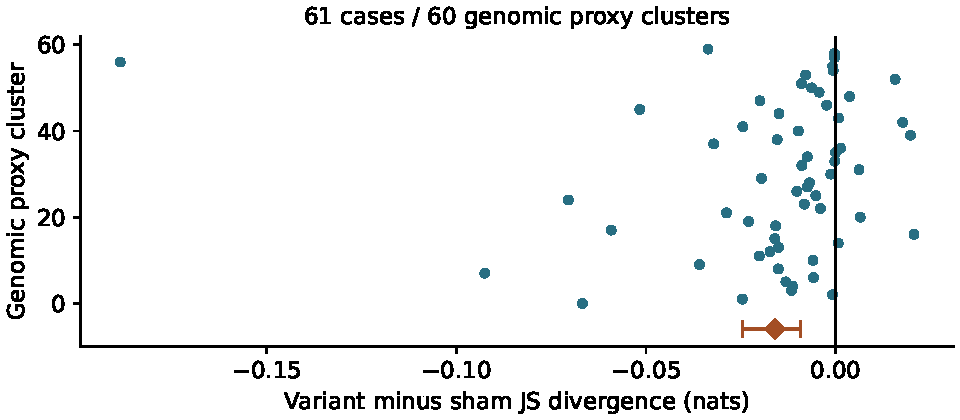
\includegraphics[width=\linewidth]{../figures/mapped_effect.pdf}
\caption{Variant-minus-sham contrasts in Jensen--Shannon divergence for 61 cases in 60 genomic proxy clusters. Blue points show cluster means in saved table order; vertical position is a display index, not a biological measurement. The diamond and bar show the equal-cluster mean and 95\% cluster-bootstrap interval in nats, conditional on the fixed checkpoint and eligibility rules.}
\label{fig:mapped}\figalttext{Scatterplot of 60 genomic cluster means for 61 mapped-query cases. Most variant-minus-sham contrasts in Jensen--Shannon divergence lie below zero. The vertical axis lists clusters in saved table order and does not encode a biological measurement. The equal-cluster mean is -0.015966 nats, with a 95 percent cluster-bootstrap interval from -0.024454 to -0.009146. Larger sham shifts fail positive differential sensitivity on this selected population; this is not a biological binding effect.}
\end{figure}

The ADASTRA archive has 512,556 records \citep{abramov2021adastra,adastra2024release}; 12,288 hash-selected scenarios were screened, 433 were motif-eligible and 61 matched/scored. The archive, screened set, motif-eligible set and scored set have distinct denominators. Original control rules retain 0/4,096 original and 1/8,192 expansion scenarios. Query matching alone retains 11 overall; removing edit-token-width matching as well yields the 61. Fifteen scored triplets have complete stable boundaries and all fifteen contrasts are negative. This stratum is a descriptive analysis performed after inspection, not an independent confirmation test.

These are reference-plus-one-SNV scenarios, not verified individual haplotypes. Symmetric JS cannot identify binding direction, and matchable cases may be unrepresentative. Segmentation, ALiBi position, context sensitivity and control differences remain alternatives. The provenance audit identifies 238 ChIP observations for 26 cases, but these form only five connected groups after shared experiments are joined. Genotype/phase, donor independence, replicate input, mapping correction and dosage remain unverified. Missing measurements are unknown, not zero. No biological correlation or biological confirmation is claimed.
\section{Discussion}
The audit provides acceptance checks for a specified component claim. Establish nucleotide and vocabulary correspondence, then check control eligibility and wiring independently of biological outcomes. A held-out effect supports contribution to the fixed readout under retained controls. Native head search requires the separately frozen endpoint to pass its sensitivity gate; binding claims require independent biological measurements and provenance. These are local acceptance rules for the implemented assays, not a validated universal evidence standard.

Table~\ref{tab:claims} separates conclusions that survive the audit from unresolved interpretations. A failed gate prevents the planned stronger claim; it does not establish that the model lacks motif information. The mapped-query result demonstrates this distinction in saved natural-variant scenarios, although the source of the larger sham effects remains unresolved.
\begin{table*}[h]\centering\small
\caption{Claim boundaries under the implemented evidence. Population sizes and uncertainty are reported with the corresponding result.}\label{tab:claims}
\begin{tabular}{p{.20\linewidth}p{.33\linewidth}p{.36\linewidth}}\toprule
Evidence & Supported conclusion & Remaining limitation \\\midrule
Correspondence & Invalid equal-index transfers can be rejected; declared maps can be certified. & Tokenizer provenance and biological adequacy require separate checks. \\
CTCF readout & A fixed selected head contributes to the specified trained output under retained controls. & Native prediction and binding effects are not established. \\
TATA readout & The retained estimate is inconclusive. & The interval permits effects in either direction. \\
Native sensitivity & Both native endpoints fail their sensitivity gates. & Failed sensitivity does not imply absence of learned motif information. \\
Biological agreement & No confirmation is claimed. & Genotype, phase, independence and measurement quality checks remain incomplete. \\\bottomrule
\end{tabular}\end{table*}


Exact-sequence, reverse-complement and short-Hamming-distance checks address specific forms of leakage, but chromosome holdout does not exclude shifted homology, indels, distant repeats or pretraining exposure. BED peak scores do not measure occupancy, and sequence entropy and run length do not identify annotated repeats. Full balance diagnostics, label specifications and failure histories accompany the supplement. The excluded Nucleotide Transformer comparison lacks established pinned loading and attention equivalence; no cross-architecture conclusion is drawn.

Original protocols, memberships, outcomes, timestamps and stopped studies are unchanged. Reporting v1 adds named Holm columns and overall sensitivity counts without model reruns. Identity-aware clustering preserves 45 CTCF and 15 TATA blocks. The source bundle links original receipts to revision \path{cc09923652f0b361f73a36f382c4358dcf8b8100} and corrected generator hashes. Compact predictions, cases, query maps, memberships, plot data and 61 raw-logit files permit offline numerical reproduction without model/genome downloads.

Earlier code snapshot mirror: \url{https://anonymous.4open.science/r/MINTS/}. Public code, the main paper, supplement and build inputs are at \url{https://github.com/ArjunCodess/MINTS}. Sequence-free reproduction data, including all 61 unchanged native logit files, are archived at \url{https://doi.org/10.5281/zenodo.23267982}. Run \texttt{python} \path{tools/verify_deposit.py} with \texttt{--data-root} pointing to the extracted dataset to verify file hashes, headline estimates, uncertainty and multiplicity corrections without model downloads. This uses saved cluster assignments; independent sequence reconstruction and fresh inference require upstream resources. Original code is MIT and original scientific outputs are CC-BY-4.0; third-party resources retain their upstream terms. No checkpoint weights, input DNA windows, full genomes or biological reads are included in the deposit.
\section{Conclusion}
MINTS checks nucleotide correspondence and diagnoses two limited control-feasibility failures. Repaired CTCF patching supports a specified trained-readout component effect; TATA remains inconclusive, and the selected CTCF head's mean base/position densities are near background. In the 61-case mapped-query study, sham divergence exceeds variant divergence and every leave-one-cluster-out mean is negative, contradicting positive differential sensitivity in this eligible population. The frozen gates remain failed. This reproducible audit does not establish general sensitivity to learned mechanisms, cross-model transfer or biological binding causality; biological measurement checks remain incomplete.
\section*{Author declarations}
Arjun Vijay Prakash is the sole author and has reviewed and approved this manuscript. The author received no funding for this work and declares no competing interests.
\bibliographystyle{oup-abbrvnat}\bibliography{references}\end{document}
